\documentclass[acmtog]{acmart}
\usepackage{graphicx}
\usepackage{subfigure}
\usepackage{natbib}
\usepackage{listings}
\usepackage{bm}

\definecolor{blve}{rgb}{0.3372549 , 0.61176471, 0.83921569}
\definecolor{gr33n}{rgb}{0.29019608, 0.7372549, 0.64705882}
\makeatletter
\lst@InstallKeywords k{class}{classstyle}\slshape{classstyle}{}ld
\makeatother
\lstset{language=C++,
	basicstyle=\ttfamily,
	keywordstyle=\color{blve}\ttfamily,
	stringstyle=\color{red}\ttfamily,
	commentstyle=\color{magenta}\ttfamily,
	morecomment=[l][\color{magenta}]{\#},
	classstyle = \bfseries\color{gr33n},
	tabsize=2
}
\lstset{basicstyle=\ttfamily}

% Title portion
\title{Assignment 4:\\ {Global Illumination}}

\author{Name:\quad Zhang Siyuan  \\ student number:\ 2019533240
\\email:\quad zhangsy3@shanghaitech.edu.cn}

% Document starts
\begin{document}
	\maketitle

	\vspace*{2 ex}

	\section{Introduction}
	\begin{itemize}
		\item Implement ray-mesh intersection test with a k-d tree and uniform-grid for acceleration by the fastest separation.
		\item Implement the ideal diffusion BRDF with an area light source.
		\item Implement the Monte-Carlo path tracing algorithm for global illumination: direct + indirect lighting.
		\item Implement the ideal specular BRDF.
	\end{itemize}
	\section{Implementation Details}
	\subsection{k-d tree}
	KD tree, also known as K-dimensional tree, is a kind of data structure that can divide K-dimensional data, and can be regarded as an extension of binary search tree, which continuously divides the dimensions in space and uses the pruning feature of search tree to reduce the time complexity, and is mainly used in multidimensional space search, such as nearest neighbor search.
	\\
	KD tree have several different separation methods, which are:

	\begin{itemize}
		\item \textbf{Standard Kd-tree Splitting Rule}
		\begin{itemize}
			\item max dimension divide
			\item max changing dimension divide
		\end{itemize}
		\item \textbf{Midpoint Splitting Rule}
		\item \textbf{Sliding Midpoint Rule}
		\item \textbf{Fair-split Rule}
		\item \textbf{Sliding Fair-split Rule}
	\end{itemize}
	I have tested several methods, and the best one is the Sliding Midpoint Rule which is very balanced for the bunny and dragon mesh.
	\begin{figure}[h]
		\centering
		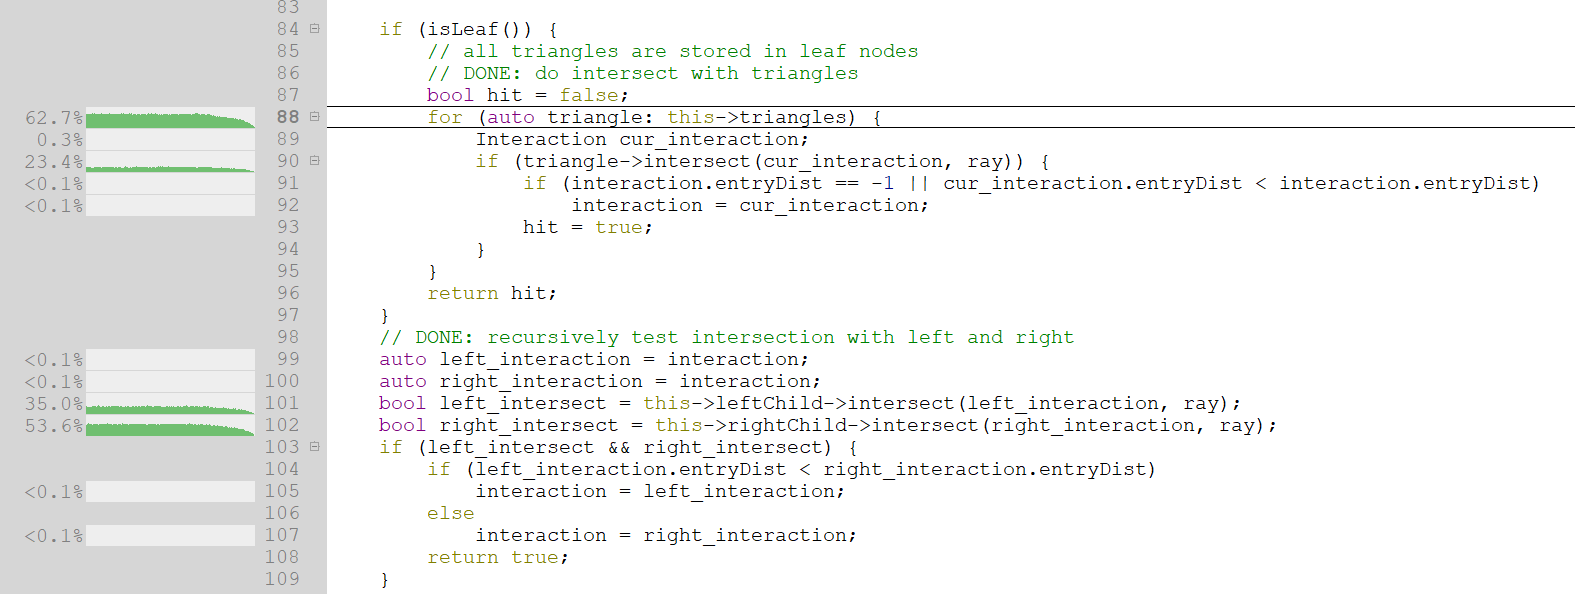
\includegraphics[width = 9cm]{HW4_kd_tree_raw.png}
		\caption{A profiling result of the ray intersection test with a k-d tree for acceleration by Standard Kd-tree Splitting Rule.}
	\end{figure}
	We can see that the when intersect rays, we spend most of the time accessing the triangles' memory which is a huge overhead.
	And when iterating the left tree and the right tree, we can see that the right tree cost as two times as the left tree.
	So that this separation method is not suitable for the bunny and dragon mesh.
	And the Sliding Midpoint Rule is well balanced as shown in the Fig 3.
	\begin{figure}[h]
		\centering
		\includegraphics[width = 9cm]{HW4_kd_tree_balanced.png}
		\caption{A profiling result of the ray intersection test with a k-d tree for acceleration by Sliding Midpoint Rule.}
	\end{figure}

	\subsection{Uniform Grid}

	While KD-tree iterates the K dimensional tree and testing whether there may have a geometry that can be hit by intersecting the bounding box, Uniform Grid just firstly assign geometries to several uniform grid and intersect the grids as shown in the fig 3.

	\begin{figure}[h]
		\centering
		\includegraphics[width = 9cm]{Uniform-Grid-2D-example.png}
		\caption{Uniform-Grid 2D example for ray intersection}
	\end{figure}

	\subsection{K-D tree VS Uniform Grid}

	After testing several times about building both of the bunny and dragon meshes, we get the following timer result

	\begin{table}[h]
		\begin{tabular}{|l|l|l|}
			\hline
			build method & Build & intersection \\ \hline
			K\_D Tree    & 1806  & 49104300     \\ \hline
			Uniform Grid & 773   & 58145300     \\ \hline
		\end{tabular}
	\end{table}

	Which shows that KD tree have a better efficiency when intersection, but the build time is doubled. So we may combine them to get better performance.

	\subsection{Light sampling}


	\[
		L(\omega_o,p) = \int _{H^2}L(\omega_i, p)f(\omega_i,\omega_o,p)\mathbf{n}\cdot\mathbf{\omega_i}\frac{\cos \theta '}{||x - x'||^2}dA
	\]
	\[
		\theta' = \angle (\omega_o, \mathbf{n})
	\]

	Sampling an area light only need to sample through two edges’ direction to get the position of sampled point.
	And the pdf returned should be $\frac{1}{A}$, where $A$ is the area of light source.


	\subsection{diffusion BRDF}
	We must first sample a reflection direction for each cameara ray. We sample the reflection direction direction using a cos-weighted technique for idea diffusion. We'll start by sampling the direction in local coordinates. We begin by sampling the unit disk uniformly.
	\[r = \sqrt{\xi_1}\]
	\[\theta = 2\pi \xi_2\]
	where $\xi_1$ and $\xi_2$ are equally distributed over the board $(0,1)$. The location on the disk is then projected onto the hemsphere.

	\[x = r \cos \theta\]
	\[y = r \sin \theta\]
	\[z = \sqrt{1 - r^2}\]

	The local coordinate is then converted to a global coordinate. In this case, we just use the Eigen library's provided function.

	Meanwhile, the Pdf value for the sampled direction can be calculated. We require $p(\omega) \propto \cos \theta$.
	\[
		\int_{H^2} c\cdot \cos \theta \mathrm{d}\omega = 1
	\]
	So for idea diffusion,
	\[
		p(\omega) = \frac{\cos \theta}{\pi} = \frac{\sqrt{1-r^2}}{\pi}
	\]
	The $f$ value must then be calculated. When considering the conservation of energy, $f = \frac{1}{2\pi} \cdot C$, where $C$ is the color of the item, the energy is spread uniformly in all directions for idea dissemination.

	\subsection{specular BRDF}
	The sampled reflection direction for concept specular reflection should be the same as the idea reflecction direction. As a result, the sampled pdf should be $1$.
	\subsection{Monte-Carlo path tracing}

	\begin{enumerate}
		\item Initialize $\beta$ = 1, $L$ = 0
		\item Generate a ray from the camera to a pixel on the image plane
		\item Compute the radiance
		\begin{enumerate}
			\item Suppose the marching ray hits at $P_i$
			\item  $L$ +=  $\beta$ * Direct lighting at $P_i$
			\item Sample ONE next ray according to $P_i$'s BRDF and find the corresponding pdf
			\item $\beta$ *=  BRDF * $cos\theta$ / pdf
			\item Spawn and march the new ray
		\end{enumerate}
	\end{enumerate}
	Just follow the given steps which is a recursive expansion.

	\section{Results}
	\begin{figure}[h]
		\centering
		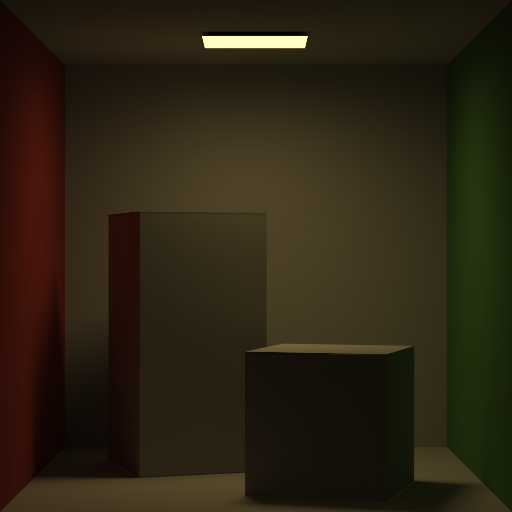
\includegraphics[height =9cm]{output_0_4096.png}
		\caption{scene 0}
	\end{figure}

	\begin{figure}[h]
		\centering
		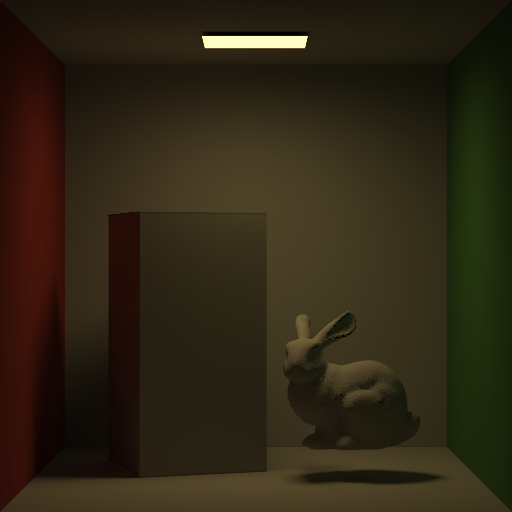
\includegraphics[height = 9cm]{output_1_4096.png}
		\caption{scene 1}
	\end{figure}

	\begin{figure}[h]
		\centering
		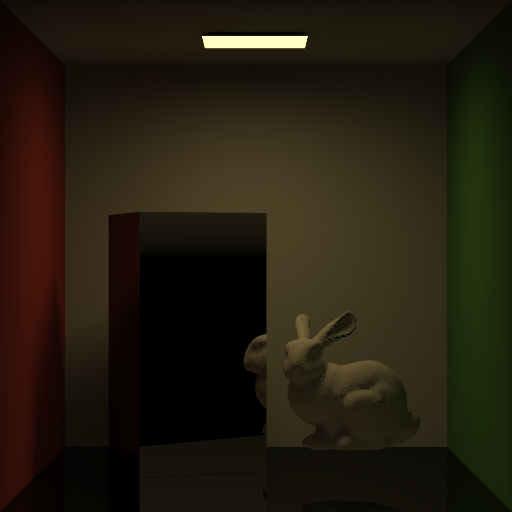
\includegraphics[height =9cm]{output_1_4096_spec.png}
		\caption{scene 1 with specular}
	\end{figure}

	\begin{figure}[h]
		\centering
		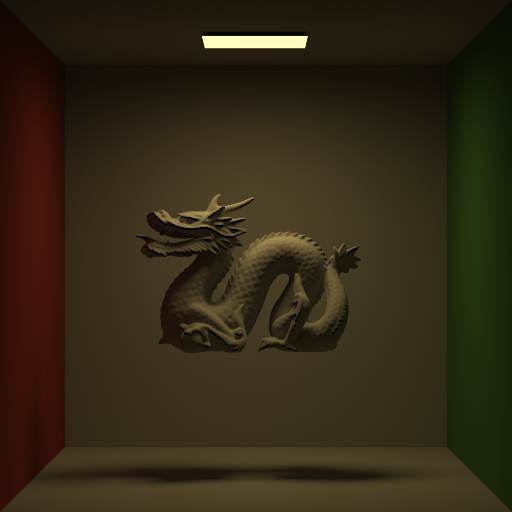
\includegraphics[height =9cm]{output_2_4096.png}
		\caption{scene 2}
	\end{figure}

	\begin{figure}[h]
		\centering
		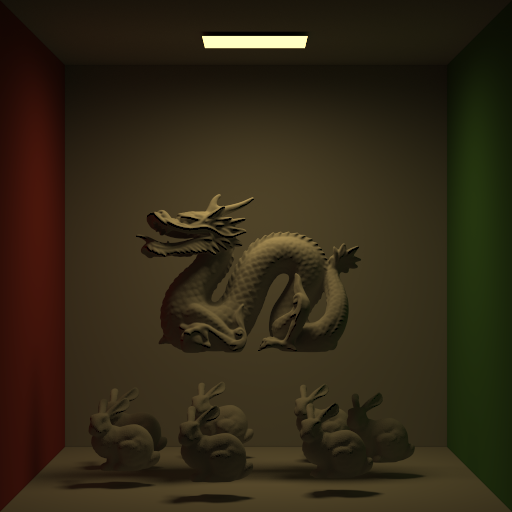
\includegraphics[height =9cm]{output_3_4096.png}
		\caption{scene 3}
	\end{figure}

	\begin{figure}[h]
		\centering
		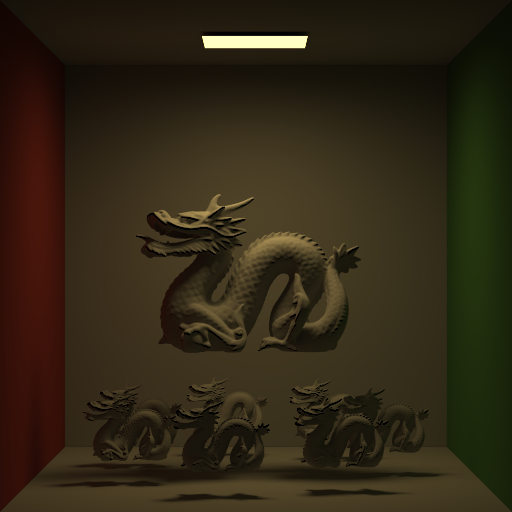
\includegraphics[height =9cm]{output_4_4096.png}
		\caption{scene 4}
	\end{figure}

\end{document}
